\documentclass[useAMS,usedcolumn,usegraphicx,usenatbib]{mn2e}
\usepackage{amssymb,amstext,amsfonts} %% ... with default font
\usepackage[fleqn]{amsmath}
\usepackage{subfigure}
\usepackage{dcolumn}
\usepackage{hyperref}

%%%%% AUTHORS - PLACE YOUR OWN MACROS HERE %%%%%
\newcommand{\eqnref}[1]{(\ref{eq:#1})}
\newcommand{\figref}[1]{fig.~\ref{fig:#1}}
\newcommand{\Figref}[1]{Figure~\ref{fig:#1}}
\newcommand{\tabref}[1]{table~\ref{tab:#1}}
\newcommand{\secref}[1]{Sec.~\ref{sec:#1}}
\newcommand{\Secref}[1]{Section~\ref{sec:#1}}
\newcommand{\apref}[1]{Appendix~\ref{sec:#1}}

\DeclareMathOperator{\Ei}{Ei}
\DeclareMathOperator{\erf}{erf}
\DeclareMathOperator{\Beta}{B}

\newcommand{\units}[1]{\ensuremath{~\mathrm{#1}}}

\newcommand{\sub}[1]{\ensuremath{_\mathrm{#1}}}
\newcommand{\super}[1]{\ensuremath{^\mathrm{#1}}}
\newcommand{\dd}{\ensuremath{\mathrm{d}}}
\newcommand{\diff}[2]{\ensuremath{\frac{\dd {#1}}{\dd {#2}}}}
\newcommand{\partialdiff}[2]{\ensuremath{\frac{\partial {#1}}{\partial {#2}}}}
\newcommand{\intd}[4]{\ensuremath{\displaystyle \int_{#1}^{#2}{#3}\,\dd{#4}}}
\newcommand{\recip}[1]{\ensuremath{\dfrac{1}{#1}}}

\newcommand{\order}[1]{\ensuremath{\mathcal{O}({#1})}}

\newcommand{\innerprod}[2]{\ensuremath{\left({#1}\middle|{#2}\right)}}
%\newcommand{\P}{\ensuremath{\mathrm{P}}}
%%%%%%%%%%%%%%%%%%%%%%%%%%%%%%%%%%%%%%%%%%%%%%%%

\title[Expectations for EMRBs from the GC]{Expectations for extreme-mass-ratio bursts from the Galactic Centre}
\author[C.\ P.\ L.\ Berry and J.\ R.\ Gair]{C.\ P.\ L.\ Berry$^{1}$\thanks{E-mail:
cplb2@cam.ac.uk}  and J.\ R.\ Gair$^{1}$\\
$^{1}$Institute of Astronomy, University of Cambridge, Madingley Road, Cambridge, CB3 0HA}

\begin{document}

\date{\today}

\pagerange{\pageref{firstpage}--\pageref{lastpage}} \pubyear{2012}

\maketitle

\label{firstpage}

\begin{abstract}
I thought I would try out the MNRAS \LaTeX{} style.
\end{abstract}

\begin{keywords}
black hole physics -- celestial mechanics -- Galaxy: centre -- gravitational waves.
\end{keywords}

\section{Introduction}

The most compelling evidence for the existence of astrophysical black holes (BHs) comes from the measurement of stellar orbits at the centre of the Galaxy. The stars are found to orbit an object of mass $M_\bullet \simeq 4 \times 10^6 M_\odot$ coincident with the compact radio source Sagittarius A* \citep{Reid2004, Ghez2008, Gillessen2009, Meyer2012}. This is the nearest member of a population of massive black holes (MBHs; \citealt{Volonteri2010}) that are believed to occupy the centre of galaxies \citep{Lynden-Bell1969, Lynden-Bell1971, Rees1984, Ferrarese2005}. The Galactic Centre is an ideal laboratory for investigating the properties of an MBH and its surrounding nuclear star cluster \citep{Genzel2010}.

One means of investigating the properties of MBHs is through gravitational waves (GWs). A stellar mass compact object (CO), such as a main sequence (MS) star, white dwarf (WD), neutron star or stellar mass BH, emits gravitational radiation as it orbits the MBH. On account of the extreme-mass-ratio between the two bodies, we can approximate the CO as moving in the background spacetime of the MBH.

A space-borne detector, such as the \textit{Laser Interferometer Space Antenna} (\textit{LISA}) or the \textit{evolved Laser Interferometer Space Antenna} (\textit{eLISA}), is designed to be able to detect GWs in the frequency range of interest for these encounters \citep{Bender1998, Danzmann2003, Jennrich2011, Amaro-Seoane2012a}. There are currently no funded space-borne detector missions. However, the European Space Agency's \textit{LISA Pathfinder} will launch in 2014 and demonstrate the key technologies required for successful space-borne mission \citep{Anza2005, Antonucci2012}.

The gravitational waveforms emitted from extreme-mass-ratio systems have been much studied \citep{Glampedakis2005, Barack2009}. The GWs carry away energy and angular momentum, causing the orbit to shrink until eventually the object plunges into the MBH. The primary focus has been upon the later stages of the orbital evolution, immediately preceding plunge. By this point, the orbit has circularised and emits continuously within the detector's frequency band. These signals are extreme mass-ratio inspirals (EMRIs; \citealt{Amaro-Seoane2007}). EMRIs can be observed over many orbits, allowing exquisitely high signal-to-noise ratios (SNRs) to accumulate. This makes them excellent probes of the background geometry.

EMRIs evolve from more eccentric orbits. These initial orbits may be the results of scattering from two-body encounters. Rather than emitting a continuously detectable signal, highly eccentric orbits only emit significant radiation in a burst around the point of closest approach to the MBH. These are extreme mass-ratio bursts (EMRBs; \citealt*{Rubbo2006}).

EMRBs are much shorter in duration than EMRIs. This means they do not accumulate as high SNRs, or produce as detailed maps of the spacetime. They are therefore less valued prizes. However, they may still be an interesting signal. As an object inspirals it emits many bursts before eventually settling into a low eccentricity EMRI. Some objects will be scattered by two-body encounters and never reach the EMRI phase \citep{Alexander2003}. Thus, there are many potential EMRBs per EMRI, although this does not necessarily translate to there being more detectable EMRBs than EMRIs.

For EMRBs to be a useful astronomical signal we require three things: the bursts contain sufficient information to improve our knowledge of their source systems; their event rate is sufficiently high that we expect to observe them over a mission life time, and the signals can be successfully extracted from the data stream.

We have previously addressed the first concern: EMRBs can give good constraints on the key parameters describing the Galaxy's MBH if the periapse distance is $r\sub{p} \lesssim 10 r\sub{g}$, where $r\sub{g} = GM_\bullet/c^2$ is a gravitational radius \citep{Berry2013}. This would allow us to improve upon the current uncertainty in the mass measurement of $8\%$ \citep{Gillessen2009}. In addition, we could also measure the spin magnitude to a precision of better than $0.1$.

The second concern shall be the subject of this work. Previously, the best estimate for the event rate was given by \citet*{Hopman2007}; they predicted the event rate for \textit{LISA} was $\sim 1\units{yr^{-1}}$. We follow a similar approach, but significantly, we improve the calculation of SNR by using numerical kludge (NK) waveforms \citep{Babak2007}. In addition to this, we extend the analysis by not only considering the number of events that would be detectable, but also how many would be informative.

\section{Waveforms and parameter uncertainties}\label{sec:Waveforms}

To establish the detectability and usefulness of EMRBs, it is necessary to calculate model waveforms. This is done using the numerical kludge approximation. We use exactly the same construction as is described in \citet{Berry2013}; the key details are outlined below.

The detectability of a burst is dependent upon its SNR. To save calculating SNRs directly, it is possible to estimate the value from the periapse radius using a simple scaling relation. This is introduced in \secref{SNR}. We make use of this when selecting orbits of potential interest, but calculate the SNR from waveforms for more accurate results.

Once we have determined which bursts are of interest, we can evaluate the accuracy to which parameters can be determined, should that burst be observed. To do so, we perform Markov chain Monte Carlo (MCMC) simulations \citep[chapter 29]{MacKay2003}.

\subsection{Numerical kludge waveforms\label{sec:NK}}

Extreme-mass-ratio signals can be simulated in a computationally efficient manner using a semirelativistic approximation \citep{Ruffini1981}: we assume the CO moves along a geodesic in the Kerr geometry, but radiates as if it were in flat spacetime. This technique is known as a numerical kludge. The justification of this technique is through comparison with more accurate, and computationally intensive, methods \citep{Gair2005, Babak2007}. The waveforms are accurate to typically a few percent \citep{Tanaka1993,Gair2005}: the error in our waveforms has been estimated as typically $\sim 5\%$, increasing to $\sim 10\%$ for the most relativistic orbits ($r\sub{p} \lesssim 4 r\sub{g}$; \citealt{Berry2013}).

To construct our NK waveforms, we first integrate the Kerr geodesic equations of motion. We only consider parabolic (marginally bound) orbits, where the orbiting body is at rest at infinity.

To avoid difficulties with turning points in the trajectory, we employ angular variables in place of the radial and polar coordinates \citep{Drasco2004}
\begin{align}
r = {} & \frac{2 r\sub{p}}{1 + \cos\psi};\\
\cos^2\theta = {} & \frac{Q}{Q+L_z^2}\cos^2\chi,
\end{align}
where $Q$ is the Carter constant and $L_z$ is the angular momentum about the $z$-axis.

Once the Kerr geodesic is constructed, we identify the Boyer-Lindquist co-ordinates with flat-space spherical polars \citep{Gair2005, Babak2007}. Using the relativistic trajectory ensures the waveform incorporates the correct frequency components; translating to flat-space means we can make use of the flat-space wave-generation formula. The downside of this is the waveform amplitude will not be precisely correct.

We use the quadrupole-octupole formula for the gravitational strain \citep{Bekenstein1973, Press1977, Yunes2008}. This is the familiar quadrupole formula (\citealt*[section 36.10]{Misner1973}; \citealt[section 17.9]{Hobson2006}), plus the next order terms. The higher order terms modify the amplitudes of some frequency components by a few tens of percent for the more relativistic orbits.

\subsection{SNR scaling\label{sec:SNR}}

The SNR $\rho$ of a particular burst depends upon the precise shape of its trajectory (as specified by initial conditions) and the position of the detector. However, the most important parameter is the periapse distance.

The $\rho$--$r\sub{p}$ relation is largely determined by the shape of the noise curve. For our simulations, we employ the noise model of \citet{Barack2004}. For bursts from the Galactic Centre, over much of the range of interest, the curve can be approximated as a simple power law \citep{Berry2013}
\begin{equation}
\log\rho \simeq -2.7\log\left(\frac{r\sub{p}}{r\sub{g}}\right) + \log\left(\frac{\mu}{M_\odot}\right) + 4.9,
\label{eq:SNR-power-law}
\end{equation}
where $\mu$ is the mass of the CO.

We assume a detection threshold of $\rho = 10$. This gives expected detection limits on the periapse radius. A $1 M_\odot$ CO should be detectable for $r\sub{p} \lesssim 27 r\sub{g}$, while a $10 M_\odot$ CO for $r\sub{p} < 65 r\sub{g}$.

\subsection{Parameter estimation}

Once we have a detected signal $\boldsymbol{s}(t)$, we can consider inference of the source parameters $\boldsymbol{\lambda}$. The waveform depends on the properties of the MBH; the CO and its orbit, and the detector.

We assume the position of the detector is known, and the MBH is coincident with the radio source of Sgr A* which is within $20 r_\mathrm{g}$ of the MBH~\citep{Reid2003,Doeleman2008}. We use the J2000.0 coordinates which are determined to high accuracy~\citep{Reid1999, Yusef-Zadeh1999}.

The parameters left to infer are:
\begin{enumerate}
\item[(1)] The MBH's mass $M_\bullet$. This is well constrained by the observation of stellar orbits about Sgr A*~\citep{Ghez2008, Gillessen2009}, we employ the estimate $M_\bullet = (4.31 \pm 0.36) \times 10^6 M_\odot$.
\item[(2)] The spin parameter $a_\ast$.
\item[(3, 4)] The orientation angles for the black hole spin $\Theta_\mathrm{K}$ and $\Phi_\mathrm{K}$.
\item[(5)] The ratio of the Galactic Centre distance and the CO mass $\zeta = R_0/\mu$. This scales the amplitude of the waveform. The distance has been measured using stellar orbits to be $R_0 = 8.33 \pm 0.35~\mathrm{kpc}$~\citep{Gillessen2009}.
\item[(6, 7)] The angular momentum of the CO, parametrized by the magnitude at infinity $L_\infty = \sqrt{L_z^2 + Q}$ and the orbital inclination $\iota = \tan^{-1}(\sqrt{Q}/L_z)$.
\item[(8--10)] Coordinates specifying the trajectory. We use the angular phases at periapse, $\phi_\mathrm{p}$ and $\chi_\mathrm{p}$, as well as the time of periapse $t_\mathrm{p}$.
\end{enumerate}

The probability the source is described by parameters $\boldsymbol{\lambda}$ is given by the posterior distribution
\begin{equation}
p(\boldsymbol{\lambda}|\boldsymbol{s}(t)) = \frac{p(\boldsymbol{s}(t)|\boldsymbol{\lambda})p(\boldsymbol{\lambda})}{p(\boldsymbol{s}(t))}.
\end{equation}
Here $p(\boldsymbol{s}(t)|\boldsymbol{\lambda})$ is the likelihood of the parameters, $p(\boldsymbol{\lambda})$ is the prior probability distribution for the parameters, and the evidence $p(\boldsymbol{s}(t))$ is a normalisation factor.

If the parameter set $\boldsymbol{\lambda}_0$ defines a waveform $\boldsymbol{h}_0(t) = \boldsymbol{h}(t; \boldsymbol{\lambda}_0)$, the likelihood of the parameters is
\begin{equation}
p(\boldsymbol{s}(t)|\boldsymbol{\lambda}_0) \propto \exp\left[-\recip{2}\innerprod{\boldsymbol{s}-\boldsymbol{h}_0}{\boldsymbol{s}-\boldsymbol{h}_0}\right].
\label{eq:likelihood}
\end{equation}
Here $\innerprod{\boldsymbol{s}-\boldsymbol{h}_0}{\boldsymbol{s}-\boldsymbol{h}_0}$ is the overlap between waveforms defined by the standard signal inner product \citep{Cutler1994}. This is the probability of the realisation of noise signal $\boldsymbol{n}(t) = \boldsymbol{s}(t) - \boldsymbol{h}_0(t)$.

To assess the accuracy to which parameters can be determined, we must find the width of the posterior distribution. MCMC methods are widely used for inference problems; they are a class of algorithms used for integrating over complicated probability distributions. Parameter space is explored by constructing randomly a chain of samples, with an acceptance rate dependent upon their probabilities \citep{Metropolis1953,Hastings1970}. The distribution of points visited by the chain maps out the underlying distribution. We employ the same semi-adaptive algorithm as was previously used in \citet{Berry2013}.

\section{Calculating event rates}

\subsection{The distribution function}

We wish to calculate the probability there is an encounter between a compact object, on an orbit described by eccentricity $e$ and periapse radius $r\sub{p}$, and the MBH. We begin by following the work of \citet{Bahcall1976, Bahcall1977} and assuming the distribution function (DF) $f$ within the Galactic core is only a function of the orbital energy \citep{Shapiro1978}. The energy per unit mass of the orbit is
\begin{equation}
\mathcal{E} = \frac{v^2}{2} - \frac{GM_\bullet}{r},
\end{equation}
where $v$ is orbital velocity. The number of stars is
\begin{equation}
N = \int \dd^3r \int \dd^3v f(\mathcal{E}).
\end{equation}
Close to the centre of the Galactic core, dynamics are dominated by the influence of the MBH as it is significantly more massive than the surrounding stars. Its radius of influence is \citep{Frank1976}
\begin{equation}
r\sub{c} = \frac{GM_\bullet}{\sigma^2},
\label{eq:r_c}
\end{equation}
where $\sigma^2$ is the line-of-sight velocity dispersion. We assume the mass of stars enclosed within $r\sub{c}$ is greater than the $M_\bullet$, which is much greater than the mass of a typical star $M_\star$ \citep{Bahcall1976}. We define a reference number density $n_\star$ from the enclosed mass $m_\ast(r)$ such that
\begin{equation}
m_\star(r\sub{c}) = \frac{4\pi r\sub{c}^3}{3}n_\star M_\star.
\end{equation}
Within the core, the DF can be calculated using the approximation of Fokker-Planck formalism \citep[section 7.4]{Binney2008}. The population of bound stars is evolved numerically until a steady state is reached: the unbound stars form a reservoir with an assumed Maxwellian distribution. Denoting a species of star by its mass $M$,
\begin{equation}
f_M(\mathcal{E}) = \frac{C_M n_\star}{(2\pi\sigma_M^2)^{3/2}} \exp\left(-\frac{\mathcal{E}}{\sigma_M^2}\right),\quad\mathcal{E} > 0,
\label{eq:Unbound_DF}
\end{equation}
where $C_M$ is a normalisation constant.\footnote{$C_M$ determines the population ratios of species $M$ far from the black hole \citep{Alexander2009}.} If different stellar species are in equipartition, as assumed by \citet{Bahcall1976, Bahcall1977}, we expect
\begin{equation}
M \sigma_M^2 = M_\star \sigma_\star^2.
\end{equation}
However, if the unbound stellar population has reached equilibrium by violent relaxation, all mass groups are expected to have similar dispersions:
\begin{equation}
\sigma_M = \sigma_\star = \sigma,
\end{equation}
and we have equipartition of energy per unit mass \citep{Lynden-Bell1967}. This is assumed here following \citet{Alexander2009} and \citet{O'Leary2009}. The steady-state DF is largely insensitive to this choice \citep{Bahcall1977, Alexander2009}.

For bound orbits, the DF can be approximated as a power law \citep{Peebles1972}
\begin{equation}
f_M(\mathcal{E}) = \frac{k_M n_\star}{(2\pi\sigma^2)^{3/2}}\left(-\frac{\mathcal{E}}{\sigma^2}\right)^{p_M},\quad\mathcal{E} < 0.
\label{eq:Bound_DF}
\end{equation}
The exponent $p_M$ varies depending upon the mass of the object, determining mass segregation. For a system with a single mass component $p = 1/4$ \citep{Bahcall1976, Young1977}. The normalisation constant $k_M$ reflects the relative abundances of the different species.\footnote{For a single mass population ($p = 1/4$) $k = 2 C$ gives a fit correct to within a factor of two \citep{Bahcall1976,Keshet2009}, we assume this holds for the dominant species of stars as, although it changes slightly with $p$, variation is small compared to errors introduced by fitting a simple power law \citep{Hopman2006, Alexander2009}.}

These cusp profiles should exist if the system has had sufficient time to become gravitationally relaxed. There is current debate about whether this may be the case, both for the Galactic centre and galaxies in general. This is discussed further in \apref{tauGC}. For concreteness, we assume a cusp has formed. If a cusp has not formed, we expect there to be a shallower core profile, with fewer objects passing close to the MBH. Our results are therefore an upper bound on possible event rates \citep{Merritt2010a,Gualandris2012}. 

\subsection{Model parameters}\label{sec:GC-Param}

We use the Fokker-Planck model of \citet{Hopman2006, Hopman2006a, Alexander2009}. This includes four stellar species: main sequence (MS) stars, white dwarfs (WDs), neutron stars (NSs), and black holes (BHs). Their properties are summarised in \tabref{HA}. The behaviour of the Fokker-Planck model has been verified by $N$-body simulations \citep{Baumgardt2004,Preto2010}.
\begin{table}
\begin{minipage}{\columnwidth}
 \centering
  \caption{Stellar model parameters for the Galactic core using the results of \citet{Alexander2009} We use the main sequence star as our reference. The number fractions for unbound stars are estimates corresponding to a model of continuous star formation \citep{Alexander2005}; \citet{O'Leary2009} arrive at the same proportions.\label{tab:HA}}
  \begin{tabular}{@{} l D{.}{.}{2.1} D{.}{.}{1.3} D{.}{.}{1.1} D{.}{.}{1.3} @{}}
  \hline
   Star & \multicolumn{1}{c}{$M/M_\odot$} & \multicolumn{1}{c}{$C_M/C_\star$} & \multicolumn{1}{c}{$p_M$} & \multicolumn{1}{c}{$k_M/k_\star$\footnote{\citet*{Toonen2009}}} \\
 \hline
 MS & 1.0 & 1 & -0.1 & 1 \\
 WD & 0.6 & 0.1 & -0.1 & 0.09 \\
 NS & 1.4 & 0.01 & 0.0 & 0.01  \\
 BH & 10 & 0.001 & 0.5 & 0.008 \\
\hline
\end{tabular}
\end{minipage}
\end{table}
The steeper power law for black holes means they segregate about the MBH.\footnote{Extrapolating, they would dominate in place of MS stars for radii $r < 10^{-4}r\sub{c}$.}

Binaries may form in the Galactic core, encouraged by its high stellar density \citep{O'Leary2009}. However the binary fraction is still expected to be small \citep{Hopman2009}. Binaries are also disrupted by the MBH for periapses smaller than
\begin{equation}
r\sub{B}  \simeq \left(\frac{M_\bullet}{M_1 + M_2}\right)^{1/3}a\sub{B},
\end{equation}
where $M_1$ and $M_2$ are the masses of the binary's components, and $a\sub{B}$ is the binary's semi-major axis [cf.\ \eqnref{Tidal} below]. Thus, we ignore the possible presence of binaries.

We assume $M_\bullet = (4.31 \pm 0.36) \times 10^6 M_\odot$ \citep{Gillessen2009} and $\sigma = (103 \pm 20)\units{km\,s^{-1}}$ \citep{Tremaine2002}. This gives a core radius of $r\sub{c} = (1.7 \pm 0.7)\units{pc}$. Using the results of \citet{Ghez2008} we would expect the total mass of stars core to be $m_\star(r\sub{c}) = 6.4 \times 10^6 M_\odot$, which is within $5\%$ of the value obtained similarly from \citet{Genzel2003}. This gives a reference stellar density of $n_\star = 2.8 \times 10^5\units{pc^{-3}}$.

\subsection{Parametrizing in terms of eccentricity \& periapsis}

We characterise orbits by their eccentricity $e$ and periapse radius $r\sub{p}$. The latter, unlike the semimajor axis, is always well defined regardless of eccentricity. For Keplerian orbits, the energy $\mathcal{E}$ and angular momentum $\mathcal{J}$ per unit mass are entirely characterised by these parameters
\begin{align}
\label{eq:Energy_ecc}
\mathcal{E} = {} & -\frac{GM_\bullet(1 - e)}{2r\sub{p}}; \quad \mathcal{J}^2 = GM_\bullet(1 + e)r\sub{p}.
\end{align}
The DF is defined per element of phase space: it is necessary to change variables from position and velocity to eccentricity and periapsis. We decompose the velocity into three orthogonal components: radial $v_r$, azimuthal $v_\phi$ and polar $v_\theta$. We assume the core is spherically symmetric \citep{Genzel2003, Schodel2007}, therefore we are only interested in the combination
\begin{equation}
v_\perp^2 = v_\phi^2 + v_\theta^2 = v^2 - v_r^2.
\end{equation}
Under this change of variables
\begin{equation}
\dd^3v = \dd v_r \dd v_\phi \dd v_\theta \rightarrow 2\pi v_\perp \,\dd v_r \,\dd v_\perp.
\end{equation}
The specific energy and angular momentum are given by
\begin{align}
\mathcal{E} = {} & \frac{v_r^2 + v_\perp^2}{2} - \frac{GM_\bullet}{r}; \quad \mathcal{J}^2 = r^2 v_\perp^2.
\end{align}
Combining these with our earlier expressions in terms of $e$ and $r\sub{p}$,
\begin{align}
v_\perp^2 = {} & \frac{GM_\bullet(1 + e)r\sub{p}}{r^2}, \\*
v_r^2 = {} & GM_\bullet\left[\frac{2}{r} - \frac{(1 - e)}{r\sub{p}} - \frac{(1 + e)r\sub{p}}{r^2}\right].
\end{align}
From the latter we can verify the turning points of an orbit occur at
\begin{equation}
r = r\sub{p}, \: \frac{1+e}{1-e}r\sub{p};
\end{equation}
the periapse is the only turning point for orbits with $e > 1$. Since we now have expressions for $\{v_r, v_\perp\}$ in terms of $\{e, r\sub{p}\}$, we can 
%calculate the Jacobian
%\begin{equation}
%\left|\frac{\partial(v_r, v_\perp)}{\partial(e, r\sub{p})}\right| = \recip{2v_rv_\perp}\frac{e}{r\sub{p}}\left(\frac{GM_\bullet}{r}\right)^2.
%\end{equation}
%Using this, we may
rewrite our velocity element as
\begin{equation}
\dd^3v \rightarrow \frac{\pi e}{v_rr\sub{p}}\left(\frac{GM_\bullet}{r}\right)^2\,\dd e \,\dd r\sub{p}.
\end{equation}
As a consequence of our assumed spherical symmetry, 
%the volume element is
%\begin{equation}
%\dd^3r = 4\pi r^2 \,\dd r.
%\end{equation}
%Thus, 
the phase space volume element can be expressed as
\begin{equation}
\dd^3r\dd^3v \rightarrow \frac{4\pi^2(GM_\bullet)^2e}{v_rr\sub{p}}\,\dd r\,\dd e \,\dd r\sub{p}.
\end{equation}
The number of stars in an element $\dd r\,\dd e\,\dd r\sub{p}$ is
\begin{equation}
n(r, e, r\sub{p}) = \frac{4\pi^2(GM_\bullet)^2e}{v_rr\sub{p}}f(\mathcal{E}).
\end{equation}

From this, we can construct the expected number of stars on orbits defined by $\{e, r\sub{p}\}$. We define this locally, allowing it to vary with position. The number of stars found in a small radius range $\delta r$ with given orbital properties is
\begin{equation}
n(r, e, r\sub{p})\delta r = N(e, r\sub{p}; r)\frac{\delta t}{P(e, r\sub{p})},
\end{equation}
where $N(e, r\sub{p}; r)$ is the total number of stars with orbits given by $\{e, r\sub{p}\}$ defined at $r$, $\delta t$ is the time spent in $\delta r$ and $P(e, r\sub{p})$ is the period of the orbit. We defer the definition of this time for unbound orbits for now. The time spent in the radius range is
\begin{equation}
\delta t = 2\frac{\delta r}{v_r},
\end{equation}
where the factor of $2$ accounts for inwards and outwards motion. Hence
\begin{align}
N(e, r\sub{p}; r) = {} & \recip{2} v_r P(e, r\sub{p}) n(r, e, r\sub{p}) \nonumber \\
 = {} & \frac{2\pi^2(GM_\bullet)^2 e P(e, r\sub{p})}{r\sub{p}}f(\mathcal{E}).
\end{align}
The right hand side is independent of position, subject to the constraint that the radius is in the allowed range for the orbit $r\sub{p} \leq r \leq (1+e)r\sub{p}/(1-e)$, and so $N(e, r\sub{p}) \equiv N(e, r\sub{p}; r)$. This is a consequence of the DF being dependent only upon a constant of the motion.\footnote{See \citet{Bahcall1976} equation (9) for a similar result.}

If a burst of radiation is emitted each time a star passes through periapse, the event rate for burst emission from orbits with parameters $\{e, r\sub{p}\}$ is given by
\begin{align}
\Gamma(e, r\sub{p}) = {} & \frac{N(e, r\sub{p})}{P(e, r\sub{p})} = \frac{2\pi^2(GM_\bullet)^2 e}{r\sub{p}}f(\mathcal{E}).
\label{eq:Gamma}
\end{align}
The orbital period drops out from the calculation, so we do not have to worry about an appropriate definition for unbound orbits.

%From the event rate we may define a probability of seeing a given number of events subject to the assumption they are uncorrelated: it is given by the Poisson distribution. The probability of there being $r$ events is
%\begin{equation}
%\Pr(r|\Gamma(e, r\sub{p})) = \frac{\Gamma^r\exp(-\Gamma)}{r!}.
%\end{equation}
%The probability of there being a burst from an orbit with periapse $r\sub{p}$ and eccentricity $e$ is hence
%\begin{equation}
%\Pr(r \neq 0|\Gamma(e, r\sub{p})) = 1 - \Pr(r = 0|\Gamma(e, r\sub{p})).
%\end{equation}

%To estimate the expectation of a quantity across all orbits we use
%\begin{equation}
%\left\langle X\right\rangle = \sum\sub{R} \int_0^\infty \dd e \int_0^\infty \dd r\sub{p} X(r;r\sub{p},e)\Pr(r|\Gamma(e, r\sub{p})).
%\end{equation}
%Since the probability decays rapidly for large $r$, we may truncate the sum to give the required level of accuracy,

To generate a representative sample for the orbital parameters $e$ and $r\sub{p}$, we use $\Gamma(e, r\sub{p})\dd e\, \dd r\sub{p}$ as the rate for a Poisson distribution.

\subsection{The inner cut-off}

From \eqnref{Gamma} we see the event rate is highly sensitive to the smallest value of the periapsis. Ultimately the orbits cannot encroach closer to the MBH than its last stable orbit. This depends upon the spin of the MBH, but is of the order of its Schwarzschild radius. Before we reach this point, there are other processes that may intervene to deplete the orbiting stars. Our treatment of these is approximate, but should produce reasonable estimates. We consider three processes: tidal disruption by the MBH; GW inspiral, and collisional disruption. Tidal disruption imposes a definite (albeit approximate) cut-off, while the others use statistical arguments. For these methods, we will need to define a reference time-scale for relaxation. This is done in \secref{Relax}, with further details found in \apref{time-scale}.

The calculated inner cut-offs for the four stellar species are shown in \figref{Cuts}.
\begin{figure*}
\begin{center}
   \subfigure[{Main sequence stars}]{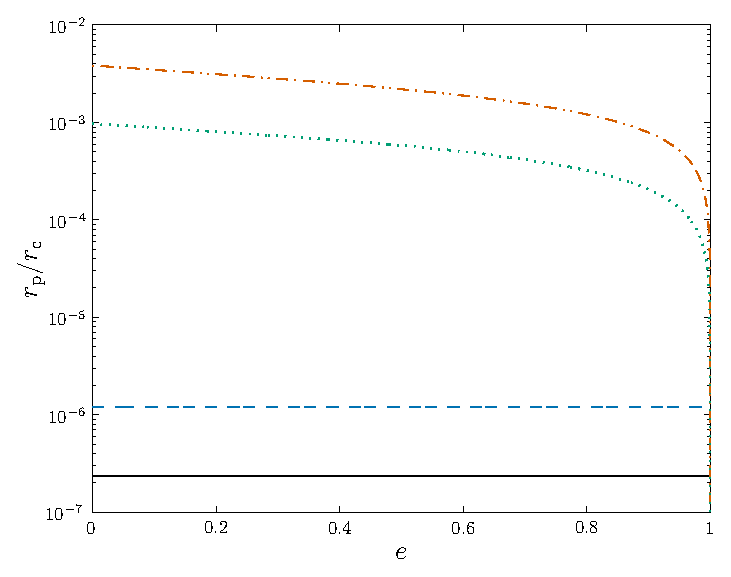
\includegraphics[width=0.4\textwidth]{Fig_Inner_cut_1.eps}} \quad 
   \subfigure[{White dwarfs}]{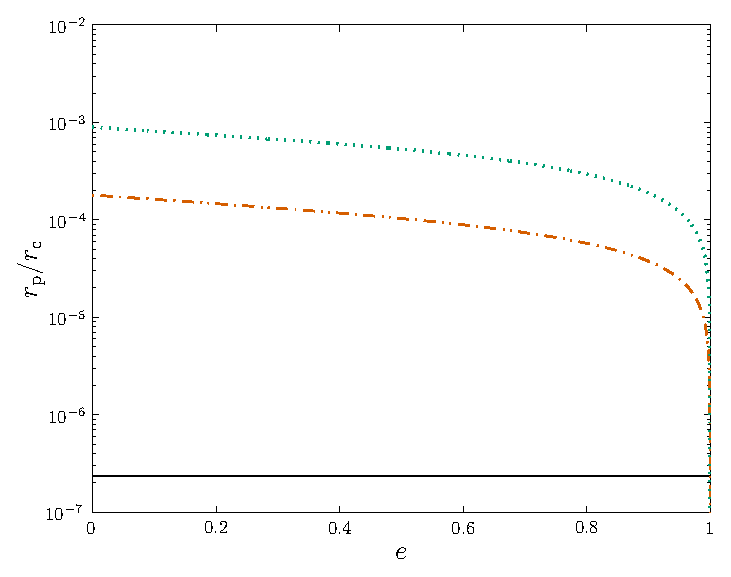
\includegraphics[width=0.4\textwidth]{Fig_Inner_cut_2.eps}} \\
   \subfigure[{Neutron stars}]{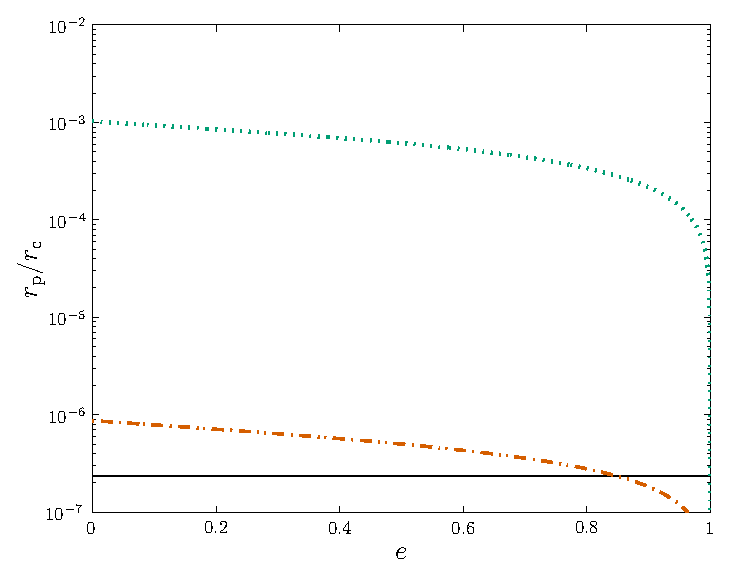
\includegraphics[width=0.4\textwidth]{Fig_Inner_cut_3.eps}} \quad
   \subfigure[{Black holes}]{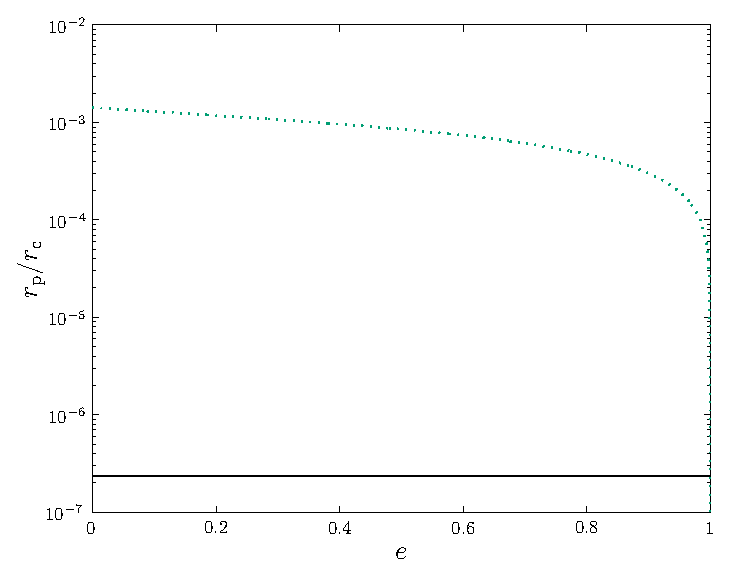
\includegraphics[width=0.4\textwidth]{Fig_Inner_cut_4.eps}}
\caption{Inner cut-off radii for the Galactic Centre as a function of eccentricity. The solid line is the Schwarzschild radius of the MBH; the dashed line is the tidal radius; the dot-dashed line is the collisional cut-off, and the dotted line is the transition to the GW-dominated inspiral regime.\label{fig:Cuts}}
  \end{center}
\end{figure*}

\subsubsection{Tidal disruption}

Tidal forces from the MBH can disrupt stars. This occurs at the tidal radius
\begin{equation}
r\sub{T} \simeq \left(\frac{M_\bullet}{M}\right)^{1/3}R_M
\label{eq:Tidal}
\end{equation}
where $R_M$ is the radius of the star \citep{Hills1975, Rees1988, Kobayashi2004}.\footnote{See \citet{Kesden2012} for a general relativistic treatment.} Any star on an orbit with $r\sub{p} < r\sub{T}$ is disrupted in the course of its orbit. Parametrizing orbits by their periapsis allows us to easily determine which stars should be disrupted. We do not include the full effects of the loss cone \citep{Frank1976, Lightman1977, Cohn1978} as these were not incorporated into the Fokker-Planck calculations \citep{Hopman2009}.\footnote{The loss cone is a region in velocity space where orbits are depleted because stars are disrupted more rapidly than they can be replenished by two-body scattering.} The effect of the loss cone should be small, only modifying the DF by a logarithmic term \citep{Lightman1977, Bahcall1977, Cohn1978}. Its effects are diluted by resonant relaxation \citep{Hopman2007,Toonen2009,Merritt2011}. Furthermore, the loss cone could be refilled by the wandering of the MBH because of perturbations from the inhomogeneities in the stellar potential \citep{Sigurdsson1997,Chatterjee2002,Merritt2007}.

Tidal disruption is significant for MS stars since they are least dense: calculated in this way, only MS stars are tidally disrupted outside of the MBH's event horizon \citep{Sigurdsson1997}. The tidal radius defines the cut-off for periapsis of high eccentricity ($e \ga 1$) orbits \citep{Lightman1977}.

\subsubsection{Relaxation time-scale}\label{sec:Relax}

The motion of a star is determined not only by the dominant influence of the central MBH, but also by the other stars. The gravitational potential of the stars may be split into two components: a smooth background representing the average distribution of stars, and statistical fluctuations from random deviations in the stellar distribution. The former only contributes to the stars' orbits: we neglect this since we are more interested in the influence of the MBH. The latter may be approximated as a series of two-body encounters. These lead to scattering, in a manner much like Brownian motion \citep{Bekenstein1992,Maoz1993,Nelson1999}.

The two-body interactions mostly lead to small deflections. Over time, these may accumulate into a significant change in the dynamics. The relaxation time-scale characterises the time taken for this to happen \citep[section 1.2.1]{Binney2008}. It therefore quantifies the time over which an orbit may be repopulated by scattering. There are a variety of definitions for the relaxation time-scale. For a system with a purely Maxwellian distribution, the time-scale has the form
\begin{equation}
\tau\sub{R}\super{Max} \simeq \kappa\frac{\sigma^3}{G^2M_\star^2 n_\star\ln\Lambda},
\label{eq:tauMaxwell}
\end{equation}
where the Coulomb logarithm is $\ln\Lambda = \ln(M_\bullet/M_\star)$ \citep{Bahcall1976}, and $\kappa$ is a dimensionless number. In his pioneering work, \citet{Chandrasekhar1941, Chandrasekhar1960} defined the time-scale as the period over which the squared change in energy was equal to the kinetic energy squared, this gives $\kappa = 9/16\sqrt{\pi} \simeq 0.32$. Subsequently, \citet{Chandrasekhar1941a} described relaxation statistically, treating fluctuations in the gravitational field probabilistically; this gives $\kappa = 9/2(2\pi)^{3/2} \simeq 0.29$. \citet{Bahcall1977} define a reference time-scale from their Boltzmann equation with $\kappa = 3/4\sqrt{8\pi} \simeq 0.15$; this is equal to the reference time-scale defined as the reciprocal of the coefficient of dynamical friction by \citet{Chandrasekhar1943a, Chandrasekhar1943}. \citet{Spitzer1958} define a reference time-scale from the gravitational Boltzmann equation of \citet{Spitzer1951} where $\kappa = \sqrt{2}/\pi \simeq 0.45$. Following \citet{Spitzer1971}, \citet[section 7.4.5]{Binney2008} estimate the time-scale from the velocity diffusion coefficient of the Fokker-Planck equation yielding $\kappa \simeq 0.34$.

All these approaches yield consistent values, suggesting, as a first approximation, any is valid. We follow the classic treatment of \citet[chapter 2]{Chandrasekhar1960} which is transparent in its assumptions, adapting from a Maxwellian distribution of velocities to one derived from the DFs \eqnref{Unbound_DF} and \eqnref{Bound_DF}. This makes the model self-consistent. Since there is uncertainty in the astrophysical parameters, we will not be concerned by small discrepancies in the numerical prefactor that result from the simplifying approximations of this approach. The derivation of the relaxation time-scale along with a discussion of its short-comings are included in \apref{time-scale}. An average time-scale for the entire system $\overline{\tau\sub{R}}$ is defined in \eqnref{system-relax}, and an average for an orbit $\left\langle\tau\sub{R}\right\rangle$ is defined in \eqnref{orbital-relax}. We defer any investigation of the consequences of using an alternative formulation for future work, as differences may well be negligible whilst the computation is complicated.

Two-body interactions lead to diffusion in both energy and angular momentum. When considering a single (bound) orbit, over a relaxation time-scale the energy changes by order of itself while the angular momentum changes by the angular momentum of a circular orbit with that energy $\mathcal{J}\sub{circ}(\mathcal{E})$ \citep{Lightman1977, Rauch1996, Hopman2005, Madigan2011}:\footnote{$\mathcal{J}\sub{circ}(\mathcal{E})$ is the maximum value for orbits of that energy.}
\begin{equation}
\left(\frac{\Delta\mathcal{E}}{\mathcal{E}}\right)^{2} \approx \left[\frac{\Delta \mathcal{J}}{\mathcal{J}\sub{circ}(\mathcal{E})}\right]^{2} \approx \frac{t}{\tau\sub{R}}.
\label{eq:diffuse-relax}
\end{equation}
We may define another angular momentum relaxation time-scale as the time taken for the angular momentum to change by order of itself \citep{Merritt2011}
\begin{align}
\tau_\mathcal{J} = {} & \left[\frac{\mathcal{J}}{\mathcal{J}\sub{circ}(\mathcal{E})}\right]^2\tau\sub{R} = \left(1 - e^2\right) \tau\sub{R}.
\label{eq:J-time}
\end{align}
This can be much shorter than the energy relaxation time-scale: diffusion in angular momentum can proceed more rapidly than diffusion in energy.

\subsubsection{Gravitational wave inspiral}\label{sec:GW-in}

Stars orbiting the MBH continually emit gravitational radiation; this carries away energy and angular momentum, causing the stars to inspiral. Using the analysis of \citet{Peters1963} and \citet{Peters1964} for Keplerian binaries, it is possible to define a characteristic inspiral time-scale from the rate of change of energy. For consistency with the relaxation time-scale, we define this as \citep{MiraldaEscude2000, Merritt2011}
\begin{equation}
\tau\sub{GW} \simeq \mathcal{E}\left\langle\diff{\mathcal{E}}{t}\right\rangle^{-1},
\label{eq:tGW-def}
\end{equation}
where the term in angular brackets is the orbit-averaged rate of energy radiation. Using \eqnref{Energy_ecc} and equation (16) of \citet{Peters1963},
\begin{align}
\tau\sub{GW} \simeq {} & \frac{5}{64}\frac{c^5r\sub{p}^4}{G^3MM_\bullet\left(M + M_\bullet\right)}\frac{(1+e)^{7/2}}{(1-e)^{1/2}} \nonumber \\*
 {} & \times {} \left(1+\frac{73}{24}e^2 + \frac{37}{96}e^4\right)^{-1} \\
 \approx {} & \frac{5}{64}\frac{c^5r\sub{p}^4}{G^3MM_\bullet^2}\frac{(1+e)^{7/2}}{(1-e)^{1/2}}\left(1+\frac{73}{24}e^2 + \frac{37}{96}e^4\right)^{-1}.
\end{align}
For comparison, the total time taken for the inspiral, if undisturbed, is given in \eqnref{Bound_inspiral}. The characteristic time-scale is a better measure of the depletion of an orbit as it only depends upon the parameters of that orbit, and not its future evolution.

The time-scale associated with changes in angular momentum is \citep{Peters1964}
\begin{align}
\tau_{\mathrm{GW},\, \mathcal{J}} \simeq {} & \mathcal{J}\left\langle\diff{\mathcal{J}}{t}\right\rangle^{-1} \\
 \simeq {} & \frac{5}{32}\frac{c^5r\sub{p}^4}{G^3MM_\bullet\left(M + M_\bullet\right)}\frac{(1+e)^{5/2}}{(1-e)^{3/2}}\left(1+\frac{7}{8}e^2\right)^{-1} \\
 \approx {} & \frac{5}{32}\frac{c^5r\sub{p}^4}{G^3MM_\bullet^2}\frac{(1+e)^{5/2}}{(1-e)^{3/2}}\left(1+\frac{7}{8}e^2\right)^{-1}.
\end{align}
This is always greater than the energy time-scale; hence, we only consider changes in energy from GW emission as important for evolution of the system \citep{Hopman2005}.

Unbound stars only undergo a single periapse passage and only radiate one burst of radiation; we therefore neglect any evolution in their orbital parameters.\footnote{Changes are only important for very high eccentricity orbits (\apref{Unbound}). These are very high energy, and exponentially suppressed because of the Boltzmann factor in \eqnref{Unbound_DF}.}

The $(1-e)^{-1/2}$ dependence of $\tau\sub{GW}$ for bound orbits connects the two regimes. The rate of change of energy goes to zero as a consequence of assuming the orbital parameters do not change over the course of an orbit. It is a valid approximation since the large mass-ratio ensures a slow evolution of the system (\apref{Unbound}).

When comparing with the relaxation time-scale we are comparing rates of change, with the shorter time-scale highlighting the more rapid process that dominates the evolution \citep{Amaro-Seoane2007}. We therefore compare $\tau\sub{GW}$ with the orbital relaxation time-scale $\tau_\mathcal{J}$ \citep{Merritt2011}. Orbits with $\tau\sub{GW} < \tau_\mathcal{J}$ become depleted by GW emission faster than they are replenished by scattering. The cusp does not extend to these orbits. Yet, these orbits are not totally depopulated as an object may pass through during its inspiral from greater periapse and eccentricity. The net effects are the distributions of MS stars, WDs and NSs at high eccentricities are relatively unchanged from their cusp states, but the BH distribution is significantly depleted.

\subsubsection{Collisions}\label{sec:Collision}

As a consequence of the high densities in the Galactic core, stars may undergo a large number of close encounters with other stars \citep{Cohn1978}. These may lead to their destruction. MS stars, WDs, and NSs may be pulled apart by tidal forces if they stray too close to a more massive object. As MS stars are diffuse, they would not tidally disrupt another star \citep{Murphy1991,Freitag2005}. Close encounters would result in some mass transfer; the cumulative effect of $20$--$30$ grazing collisions could destroy a MS star \citep{Freitag2006}. The number of collisions a star undergoes in a time interval $\delta t$ is
\begin{equation}
\delta K = n(r) A v(r,e,r\sub{p})\delta t,
\end{equation}
where $A$ is the collisional cross-sectional area. For tidal disruption, where the encounter is with a collapsed object (WD, NS or BH), we set $A = \pi r_{\mathrm{T},\,{M'}}^2$, where $r_{\mathrm{T},\,{M'}}$ is the appropriate tidal radius: like \eqnref{Tidal} but with $M_\bullet$ replaced with the mass of the collapsed object $M'$. For collisions between MS stars, the cross-sectional area is simply the geometric $A = \pi R_\star^2$.\footnote{Here we assume the relative velocity of the colliding stars is much greater than the escape velocity of the star so we may neglect the effects of gravitational focusing.}

For circular orbits we can find the radius at which collisions lead to disruptions by setting $\delta K = 1$ for tidal disruption or $\delta K = 20$ for grazing collisions, and $\delta t = \overline{\tau_\mathrm{R,\,M}}$. We use the system average relaxation time-scale for the species of mass $M$ as this is the time over which stars are replenished from the reservoir. For non-circular orbits we must consider variation with position. Using $\delta r = v_r \delta t$, and then converting to an integral, for bound orbits
\begin{equation}
K = 2 A \frac{\tau\sub{R}}{P(r\sub{p},e)}\intd{r\sub{p}}{(1+e)r\sub{p}/(1-e)}{n(r)\frac{v(r,e,r\sub{p})}{v_r(r,e,r\sub{p})}}{r},
\end{equation}
where $P$ is the period of the orbit. Again we set $K = 1$ or $K = 20$ to find the orbits for which stars will be disrupted within $\overline{\tau_\mathrm{R,\,M}}$. For unbound orbits we are only interested in stars that would become disrupted before their periapse passage, so
\begin{equation}
K = A \intd{r\sub{p}}{r\sub{c}}{n(r)\frac{v(r,e,r\sub{p})}{v_r(r,e,r\sub{p})}}{r},
\end{equation}
assuming the stars in the reservoir external to the core are unlikely to undergo close collisions.

Collisions provide the cut-off for bound MS stars, and are significant for bound WDs.

\section{Results}

\subsection{Number of events}

As a first approximation for the number of events expected in a $2\units{yr}$ mission lifetime, we numerically integrated the event rate. This estimate is denoted as $\mathcal{N}_2\super{int}$. The lower limit on $r\sub{p}$ was set to be the largest of the tidal cut-off, the collisional cut-off or the MBH's Schwarzschild radius; the upper limit was the detection threshold as determined from \eqnref{SNR-power-law}. The lower bound on eccentricity was set to $0.9$, below which we do not trust the parabolic approximation for burst waveforms; since the DF decays exponentially with eccentricity for unbound orbits, the upper limit does not influence our results.

To obtain a more accurate estimate, we  performed $20000$ mission realisations. For each mission, we randomly selected a set of parameters to describe the MBH, and then picked orbits with probabilities defined by their event rates. The SNR of the resulting bursts were calculated (with the detector in a position corresponding to a random time), and a detection was recorded if $\rho > 10$. By averaging the number of events per mission, we can estimate the expected number of bursts we would expect to detect. This is denoted $\mathcal{N}_2\super{run}$.

The calculated numbers of events are shown in \tabref{Rates}.
\begin{table}
\begin{minipage}{\columnwidth}
 \centering
  \caption{Expected number of events.\label{tab:Rates}}
  \begin{tabular}{@{} l D{,}{\times}{3.4} D{,}{\times}{3.4} @{}}
  \hline
   Star & \multicolumn{1}{c}{$\mathcal{N}_2\super{int}$} & \multicolumn{1}{c}{$\mathcal{N}_2\super{run}$} \\
 \hline
 MS & 9.5,10^{-4} & 1.3,10^{-3} \\
 WD & 1.0,10^{-2} & 1.0,10^{-2} \\
 NS & 5.0,10^{-1} & 5.0,10^{-1}  \\
 BH & 1.2,10^{0} & 1.2,10^{0} \\
\hline
Total & 1.7,10^{0} & 1.7,10^{0} \\
\hline
\end{tabular}
\end{minipage}
\end{table}
The overall rates are similar to those presented in \citet{Hopman2007}. The MS rate is lower because of a larger collisional cut-off. This also influences the WD rate, however the overall rate is little changed. The NS rate is enhanced because of the inclusion of bursts from inspiralling objects. The physics for BHs is least changed, the (small) difference in event rate is partly a consequence of our more realistic SNRs. Only MS stars have a non-negligible (relative) contribution from unbound orbits.

Only BHs and NSs contribute to the event rate significantly.

\section*{Acknowledgments}
The authors are grateful for insightful discussions with Sverre Aarseth. The authors thank Tal Alexander and Clovis Hopman for useful correspondence. CPLB is supported by STFC. JRG is supported by the Royal Society.

\bibliographystyle{mn3e}
\bibliography{Galactic}

\appendix

\begin{onecolumn}

\section{Chandrasekhar's relaxation time-scale}\label{sec:time-scale}

\citet[chapter 2]{Chandrasekhar1960} defined a relaxation time-scale for a stellar system by approximating the fluctuations in the stellar gravitational potential as a series of two-body encounters. The time over which the squared change in energy is equal to the squared (initial) kinetic energy of the star is the time taken for relaxation. Relaxation is mediated by dynamical friction (\citealt{Chandrasekhar1943a}; \citealt[section 1.2]{Binney2008}). This can be understood as the drag induced on a star by the over-density of field stars deflected by its passage \citep{Mulder1983}. In the interaction between the star and its gravitational wake, energy and momentum are exchanged, accelerating some stars, decelerating others.

Chandrasekhar's approach has proved exceedingly successful despite the number of simplifying assumptions inherent in the model which are not strictly applicable to systems such as the Galactic core. We will not attempt to fix these deficiencies; the only modification is to substitute the velocity distribution.

Other authors have built upon the work of Chandrasekhar by considering inhomogeneous stellar distributions, via perturbation theory \citep{Lynden-Bell1972,Tremaine1984,Weinberg1986}; modelling energy transfer as anomalous dispersion, which adds higher order moments to the transfer probability \citep{Bar-Or2012}, or using the tools of linear response theory and the fluctuation-dissipation theory \citep[chapter 7]{Landau1958}, which allows relaxation of certain assumptions, such as homogeneity \citep{Bekenstein1992,Maoz1993,Nelson1999}. We will not attempt to employ such sophisticated techniques at this stage.

\subsection{Chandrasekhar's derivation of the change in energy}\label{sec:Chandra}

We consider the interaction of a field star, denoted by 1, with a test star, 2; the change in energy squared from interaction in time $\delta t$ is approximately \citep[chapter 2]{Chandrasekhar1960}
\begin{equation}
\Delta E^2(v_1) \simeq \frac{8\pi}{3} n(v_1)G^2m_1^2 m_2^2\ln\left(qv_2^2\right)\left\{\begin{array}{lr}\dfrac{v_1^2}{v_2} & v_1 \leq v_2\\ \dfrac{v_2^2}{v_1} & v_1 \geq v_2 \end{array}\right\}\,\dd v_1\delta t.
\end{equation}
Here $v_1$ and $v_2$ are the initial velocities, and $m_1$ and $m_2$ are the masses. $n(v_1)$ is the number of stars per velocity element $\dd v_1$; this is calculated assuming the density of stars is uniform.\footnote{The error introduced by this assumption can be partially absorbed by the appropriate choice of the Coloumb logarithm, which shall be introduced later~\citep{Just2011}.} The logarithmic term includes
\begin{equation}
q = \frac{D_0}{G\left(m_1+m_2\right)},
\end{equation}
where $D_0$ is the maximum impact parameter \citep{Weinberg1986}. To eliminate the dependence upon $v_1$ requires a specific form for the velocity distribution.

\subsection{Velocity distributions}

The velocity space DF can be obtained by integrating out the spatial dependence in the full DF. As we are restricting our attention to the core and assuming spherical symmetry
\begin{equation}
f(v) = 4\pi\intd{0}{r\sub{c}}{r^2f(\mathcal{E})}{r},
\end{equation}
where $r\sub{c}$ is defined by \eqnref{r_c}.

The DF for unbound stars is assumed to be Maxwellian as in \eqnref{Unbound_DF}. Performing the integral
\begin{align}
f_{\mathrm{u},\,M}(v) = {} & \frac{N_\ast}{\left(2\pi\sigma^2\right)^{3/2}}C_M\epsilon\left(\frac{v^2}{2\sigma^2}\right),
\end{align}
introducing
\begin{equation}
\epsilon(w) = \recip{2}\left\{\exp(-w)\left[4\exp(1) + \Ei(w) - \Ei(1)\right] - \frac{2 + w + w^2}{w^3}\right\},
\end{equation}
where $\Ei(x)$ is the exponential integral.

The DF for bound stars is approximated as a simple power law as in \eqnref{Bound_DF}. The integral gives
\begin{equation}
f_{\mathrm{b},\,M}(v) = \frac{N_\ast}{\left(2\pi\sigma^2\right)^{3/2}}k_M \left(\frac{v^2}{2\sigma^2}\right)^{p_M - 3}\begin{cases}
3 \Beta\left(\dfrac{v^2}{2\sigma^2}; 3 - p_M, 1 + p_M\right) & \dfrac{v^2}{2\sigma^2} \leq 1 \\
3 \Beta\left(3 - p_M, 1 + p_M\right) & \dfrac{v^2}{2\sigma^2} \geq 1
\end{cases},
\end{equation}
where $\Beta(x;a,b)$ is the incomplete beta function \citep[8.17]{Olver2010}, $\Beta(a,b) \equiv \Beta(1,a,b)$ is the complete beta function.

The velocity space density is related to the DF by
\begin{equation}
\frac{4\pi r\sub{c}^3}{3}n_M(v_1) = 4\pi v_1^2\left[f_{\mathrm{u},\,M}(v_1) + f_{\mathrm{b},\,M}(v_1)\right].
\end{equation}

\subsection{Defining the relaxation time-scale}

Using the specific forms for the velocity space density, we can calculate $\Delta E^2$. The functional form depends upon the velocity of the test star. If $v_2^2/2\sigma^2 < 1$, then
\begin{align}
\Delta E^2 \simeq {} & \frac{16}{3}\sqrt{2\pi}\frac{G^2m_1^2 m_2^2n_\ast}{\sigma^3}\ln\left(qv_2^2\right) \left(\frac{v_2^2}{2\sigma^2}\right) \left[k \frac{3}{(2 - p)(1 + p)}{_3F_2}\left(-1-p,2-p,\frac{3}{2};3-p,\frac{5}{2};\frac{v_2^2}{2\sigma^2}\right) + C\right]\,\delta t,
\end{align}
where ${_3F_2}(a_1,a_2,a_3;b_1,b_2;x)$ is a generalised hypergeometric function \citep[section 16]{Olver2010}.\footnote{We have suppressed subscript $M$ for brevity.} The contribution from bound and unbound stars can be identified by the coefficients $k$ and $C$ respectively. It is necessary to sum over all the species to get the total value.

If $v_2^2/2\sigma^2 > 1$,
\begin{equation}
\Delta E^2 \simeq \frac{16}{3}\sqrt{2\pi}G^2m_1^2 m_2^2n_\ast\sigma\ln\left(qv_2^2\right) \left(\frac{v_2^2}{2\sigma^2}\right)^{-1/2} \left[k\beta\left(\frac{v_2^2}{2\sigma^2};p\right) + C\alpha\left(\frac{v_2^2}{2\sigma^2}\right)\right]\,\delta t,
\end{equation}
where
\begin{align}
\alpha(w) = {} & \recip{2}\left\{3w^{-1/2} + 5 + \left[4\exp(1) - \Ei(1) + \Ei(w)\right]\left[\frac{3\sqrt{\pi}}{4}\erf\left(w^{1/2}\right) - \frac{3}{2}w^{1/2}\exp(-w)\right] - 3\sqrt{\pi}\exp(1)\erf(1) \right. \nonumber\\*
 & + \left. 3\left[{_2F_2}\left(\frac{1}{2},1;\frac{3}{2},\frac{3}{2};1\right) - w^{1/2}{_2F_2}\left(\frac{1}{2},1;\frac{3}{2},\frac{3}{2};w\right)\right]\right\}; \\
\beta(w;p) = {} & \begin{cases} \dfrac{3}{1/2 - p}\left[\Beta\left(\dfrac{5}{2},1+p\right) - \dfrac{3w^{p-1/2}}{2(2-p)}\Beta\left(3-p,1+p\right)\right] & p < \recip{2} \\
\dfrac{\pi}{32}\left[12 \ln(2) - 1 + 6 \ln(w)\right] & p = \recip{2} \end{cases} . 
\end{align}
The generalised hypergeometric function originates from the integral
\begin{equation}
\intd{}{w}{\frac{\exp(w')\erf\left({w'}^{1/2}\right)}{w'}}{w'} = \frac{4w^{1/2}}{\sqrt{\pi}}{_2F_2}\left(\frac{1}{2},1;\frac{3}{2},\frac{3}{2};w\right).
\end{equation}

Combining the two regimes, we simplify using approximate forms. For the bound contribution 
\begin{align}
\Delta E\sub{b}^2 \approx {} & 16\sqrt{2\pi}G^2m_1^2m_2^2n_\ast\sigma\ln\left(qv_2^2\right) k \gamma\left(\frac{v_2^2}{2\sigma^2};p\right)\,\delta t,
\label{eq:Bound-approx}
\end{align}
where
\begin{align}
\gamma(w;p) = {} & \left(1 + w^4\right)^{-1}\left\{\left[\dfrac{3}{(1 + p)(2 - p)}w - \dfrac{9}{5(3-p)}w^2 + \dfrac{9p}{14(7-p)}w^3 \right] + w^{7/2}\beta\left(w;p\right)\right\}.
\end{align}
The resulting error, ignoring variation from $\ln\left(qv_2^2\right)$, is less than $3\%$.

The unbound contribution is
\begin{equation}
\Delta E\sub{u}^2 \approx \frac{16}{3}\sqrt{2\pi}G^2m_1^2m_2^2n_\ast\sigma\ln\left(qv_2^2\right) C \Xi\left(\frac{v_2^2}{2\sigma^2}\right)\left[\Xi^2 + \left(\frac{v_2^2}{2\sigma^2}\right)^3\right]^{-1/2}\,\delta t,
\label{eq:Unbound-approx}
\end{equation}
where
\begin{equation}
\Xi = \lim_{w \rightarrow \infty}\left\{\alpha(w)\right\} \simeq 4.31.
\end{equation}
This reproduces the full function to better than $5\%$, ignoring variation from $\ln\left(qv_2^2\right)$.

The relaxation time-scale is the time interval $\delta t$ over which the squared change in energy becomes equal to the kinetic energy of the test star squared \citep{Bar-Or2012}
\begin{align}
\tau\sub{R} = {} & \left(\frac{m_2v_2^2}{2}\right)^2\frac{\delta t}{\Delta E^2} \\
 \approx {} & \frac{3v_2^4}{16\sqrt{2\pi}G^2n_\ast\sigma\ln\left(qv_2^2\right)} \left(\sum_M M^2 \left\{k_M \gamma\left(\frac{v_2^2}{2\sigma^2};p_M\right) + C_M\Xi\left(\frac{v_2^2}{2\sigma^2}\right)\left[\Xi^2 + \left(\frac{v_2^2}{2\sigma^2}\right)^3\right]^{-1/2}\right\}\right)^{-1}.
\label{eq:tau_R1}
\end{align}

\subsection{Averaged time-scale}

The relaxation time-scale \eqnref{tau_R1} is for a particular velocity $v_2$. This is not of much use to describe the core or even a (non-circular) orbit where there is a velocity range. It is necessary to calculate an average. Both the change in energy squared and the kinetic energy are averaged. We use two averages: over the distribution of bound velocities to give the relaxation time-scale for the system, and over a single orbit. The former is of use when considering the inner cut-off of stars due to collisions, the latter when considering the transition to GW inspiral.

\subsubsection{System relaxation time-scale}\label{sec:system-ave}

The total number of bound stars in the core is
\begin{equation}
N_{\mathrm{b},\,M} = \frac{3}{3/2 - p_M}\frac{\Gamma(p_M + 1)}{\Gamma(p_M + 7/2)}N_\ast k_M,
\end{equation}
where $\Gamma(x)$ is the gamma function. Using this as a normalisation constant, the probability of a bound star having a velocity in the range $v \rightarrow v + \dd v$ is
\begin{align}
4\pi v^2 p_{\mathrm{b},\,M}(v) \,\dd v = {} & \sqrt{\frac{2}{\pi}} \frac{v^2}{\sigma^3} \frac{\left(3/2 - p_M\right)\Gamma(p_M + 7/2)}{\Gamma(p_M + 1)} \left(\frac{v^2}{2\sigma^2}\right)^{p_M - 3}\left\{\begin{array}{lr}
\Beta\left(\dfrac{v^2}{2\sigma^2}; 3 - p_M, 1 + p_M\right) & \dfrac{v^2}{2\sigma^2} \leq 1 \\
\Beta\left(3 - p_M, 1 + p_M\right) & \dfrac{v^2}{2\sigma^2} \geq 1\end{array}\right\}\,\dd v.
\end{align}
The mean squared velocity for bound stars in the core is then
\begin{align}
\overline{v^2_{M}} = {} & 3\sigma^2\frac{3/2 - p_M}{1/2 - p_M},
\end{align}
assuming $p_M < 1/2$.

In the case $p_M = 1/2$ we encounter a logarithmic divergence. This reflects there being a physical cut-off.\footnote{A similar diverge necessitates the introduction of $D_0$ in \secref{Chandra}.} We use $v\sub{max} = c/2$, which is the maximum speed reached on a bound orbit about a Schwarzschild BH. Marginally higher speeds can be reached for prograde orbits about a Kerr BH, but the maximal velocity for retrograde orbits is marginally lower. In reality, we expect the maximum velocity to be lower due to a depletion of orbits. We also suspect a simple Newtonian description of these orbits is imprecise, but a full relativistic description is beyond this simple analysis. For $p_M = 1/2$,
\begin{align}
\overline{v^2_{M}} = {} & \frac{\sigma^2}{2}\left[12\ln(2) - 5 + 6 \ln\left(\frac{v\sub{max}^2}{2\sigma^2}\right)\right].
\end{align}
Using a typical value of $\sigma = 10^5\units{m\,s^{-1}}$,
\begin{equation}
\overline{v^2_{M}} \simeq 43\sigma^2.
\end{equation}
The mean squared velocity is an order of magnitude greater than for a Maxwellian distribution.

For the average of $\Delta E^2$, we replace $\ln\left(qv_2^2\right)$ by a suitable average so it may be moved outside the integral \citep[chapter 2]{Chandrasekhar1960}. We replace it by the Coulomb logarithm \citep{Bahcall1976}
\begin{equation}
\ln\left(q\overline{v_2^2}\right) = \ln \Lambda_M \simeq \ln\left(\frac{M_\bullet}{M}\right).
\end{equation}
\citet{Just2011} find an extremely similar result fitting a Bahcall--Wolf cusp self-consistently. We calculate the averages for the bound and unbound contributions individually. We must distinguish between the bound population of field stars and the distribution of test stars over which we are averaging. We use subscripts $M$ and $M'$ respectively.\footnote{For masses: $m_M \equiv M$, $m_{M'} \equiv M'$.} The bound average may be approximated to about $10\%$ accuracy as
\begin{align}
\overline{\Delta E^2_{\mathrm{b},\,M'}} \approx {} & \sum_M\frac{2^{11/2}}{3}G^2M^2{M'}^2n_\ast\sigma\ln\left(\Lambda_{M'}\right) k_M \frac{(3/2 - p_{M'})\Gamma(p_{M'} + 7/2)}{\Gamma(p_{M'} + 1)} \left\{ \recip{210}\left[30 + 36p_M + 25p_M^2 - p_{M'}\left(13 + 15p_M + 7 p_M^2\right) \right. \right. \nonumber \\* 
 {} & + \left. \left. p_{M'}^2\left(6 + 9p_M + 8p_M^2\right)\right]  \vphantom{\recip{210}} + \iota \left(p_M,p_{M'}\right) \right\} \delta t,
\end{align}
introducing
\begin{equation}
\iota\left(p_M,p_{M'}\right) = \Beta\left(3-p_{M'},1+p_{M'}\right) \begin{cases} \dfrac{3}{1/2 - p_M}\left[\dfrac{\Beta\left(5/2,1+p_M\right)}{2-p_{M'}} - \dfrac{3\Beta\left(3-p_M,1+p_M\right)}{2\left(2-p_M\right)\left(5/2 - p_M - p_{M'}\right)}\right] & p_M < \recip{2} \\
\dfrac{\pi}{32}\dfrac{4 + p_{M'} + 12 \left(2 - p_{M'}\right) \ln(2)}{\left(2-p_{M'}\right)^2} & p_M = \recip{2} \end{cases}.
\end{equation}

The unbound component is approximately
\begin{align}
\overline{\Delta E^2_{\mathrm{u},\,M'}} \approx {} & \sum_M\frac{2^{11/2}}{3}G^2M^2{M'}^2n_\ast\sigma\ln\left(\Lambda_{M'}\right) C_M \frac{(3/2 - p_{M'})\Gamma(p_{M'} + 7/2)}{\Gamma(p_{M'} + 1)} \nonumber \\
  & \times \left[\nu\left(p_{M'}\right) + \Xi\frac{\Beta\left(3-p_{M'},1+p_{M'}\right)}{2-p_{M'}}{_2F_1}\left(\recip{2},\frac{2-p_{M'}}{3};\frac{5-p_{M'}}{3};-\Xi^2\right) \right] \delta t,
\end{align}
where
\begin{equation}
\nu(p) = \begin{cases} \recip{1/2 - p}\left[\Beta\left(\dfrac{5}{2},1+p\right) - \Beta\left(3-p,1+p\right)\right] & p < \recip{2} \\
\dfrac{\pi}{96}\left[12 \ln(2) - 5\right] & p = \recip{2}
\end{cases} \; ,
\end{equation}
and we have used another hypergeometric function \citep[15.6.1]{Olver2010}. For consistency with the bound case we have continued to use subscript $M'$. 

The total relaxation time for a species is
\begin{align}
\overline{\tau_{\mathrm{R,}\,M'}} = {} & \left(\frac{{M'}\overline{v_{M'}^2}}{2}\right)^2\frac{\delta t}{\overline{\Delta E^2_{\mathrm{b},\,M'}} + \overline{\Delta E^2_{\mathrm{u},\,M'}}} \\
 \approx {} & \frac{3}{2^{15/2}}\frac{\Gamma(p_{M'} + 1)}{(3/2 - p_{M'})\Gamma(p_{M'} + 7/2)}\frac{\overline{v_{M'}^2}^2}{G^2n_\ast\sigma\ln\left(\Lambda_{M'}\right)} \nonumber \\* 
  & \times {} \left\{\sum_M k_M M^2 \left[ \frac{30 + 36p_M + 25p_M^2 - p_{M'}\left(13 + 15p_M + 7 p_M^2\right) + p_{M'}^2\left(6 + 9p_M + 8p_M^2\right)}{210} + \iota \left(p_M,p_{M'}\right)\right] \right. \nonumber \\*
  & + \left. \vphantom{ \left[ \frac{p_{M'}^2\left(6 + 9p_M + 8p_M^2\right)}{210}\right]} C_M M^2 \left[\nu\left(p_{M'}\right) + \Xi\frac{\Beta\left(3-p_{M'},1+p_{M'}\right)}{2-p_{M'}}{_2F_1}\left(\recip{2},\frac{2-p_{M'}}{3};\frac{5-p_{M'}}{3};-\Xi^2\right)\right]\right\}^{-1}.
\end{align}
Combining these to form an average for the entire system gives
\begin{equation}
\overline{\tau_{\mathrm{R}}} = \frac{\sum_{M'}N_{\mathrm{b,}\,M'}\overline{\tau_{\mathrm{R,}\,M'}}}{\sum_{M}N_{\mathrm{b,}\,M}}.
\label{eq:system-relax}
\end{equation}
The relaxation time-scale for individual components is used in determining the collisional cut-off as described in \secref{Collision}.

\subsubsection{Orbital average}\label{sec:orbital-ave}

We calculate the time-scale for an orbit, parametrized by $e$ and $r\sub{p}$, by averaging over one period.\footnote{We only consider bound orbits. The orbital relaxation time-scale is compared against the GW time-scale; the evolution of unbound orbits due to GW emission is negligible.} The mean squared velocity is
\begin{equation}
\left\langle v^2\left(e,r\sub{p}\right)\right\rangle = \frac{GM_\bullet(1 - e)}{r\sub{p}}.
\end{equation}
The orbital average is calculated according to \citep[section 2.2b]{Spitzer1987}
\begin{equation}
\left\langle X\right\rangle = \recip{T}\intd{0}{T}{X(t)}{t},
\end{equation}
where $T$ is the orbital period. Despite our best efforts, we have been unsuccessful at obtaining analytic forms for the averaged changes in energy squared. Therefore we compute them numerically. Switching to orbital phase angle $\vartheta$, we define
\begin{align}
I\sub{b}(e,\varrho,p) = {} & \intd{0}{\pi}{\recip{(1 + e \cos\vartheta)^2}\gamma\left(\frac{1}{2(1+e)\rho}\left(1+e^2+2e\cos\vartheta\right);p\right)}{\vartheta} \\
I\sub{u}(e,\varrho,\Xi) = {} & \intd{0}{\pi}{\frac{\Xi}{(1 + e \cos\vartheta)^2}\left[\frac{1}{2(1+e)\rho}\left(1+e^2+2e\cos\vartheta\right)\right]\left\{\Xi^2 + \left[\frac{1}{2(1+e)\rho}\left(1+e^2+2e\cos\vartheta\right)\right]^3\right\}^{-1/2}}{\vartheta}.
\end{align}
The orbital relaxation time-scale is then
\begin{align}
\left\langle\tau_{\mathrm{R},\,M'}\left(e,r\sub{p}\right)\right\rangle = {} & \left(\frac{GM_\bullet(1 - e)M'}{2r\sub{p}}\right)^2\frac{\delta t}{\left\langle\Delta E^2_{\mathrm{b},\,M'}\right\rangle + \left\langle\Delta E^2_{\mathrm{u},\,M'}\right\rangle} \\
 \approx {} & \frac{3}{64}\sqrt{\frac{\pi}{2}} \frac{M_\bullet^2(1 - e)^{1/2}}{n_\ast \sigma r\sub{p}^2(1 + e)^{3/2}\ln\left(\Lambda_{M'}\right)} \left[\sum_M k_M M^2 I\sub{b}\left(e,\frac{r\sub{p}}{r\sub{c}},p_M\right) + C_M M^2 I\sub{u}\left(e,\frac{r\sub{p}}{r\sub{c}},\Xi\right)\right]^{-1}.
\label{eq:orbital-relax}
\end{align}
This time-scale is defined similarly to the inspiral time-scale \eqnref{tGW-def}.

Diffusion in angular momentum proceeds over a shorter time, as defined by \eqnref{J-time}. Combining this with \eqnref{orbital-relax} gives the orbital angular momentum relaxation time-scale.

\subsection{Discussion of applicability}

In deriving the relaxation time-scales it has been necessary to make a number of approximations, both mathematical and physical. We have been careful to ensure that the inaccuracies introduced are of the order of a few percent, and subdominant to the errors inherent from the physical assumptions and uncertainties in astronomical quantities. There are two key physical approximations that may limit the validity of the results.

First, it was assumed  the density of stars was uniform. This is a pragmatic assumption necessary to perform integrals over impact parameter and angular orientation. It is not the case that density in the core is uniform. However, this approximation is not as bad as it first may seem. As a star travels on its orbit it moves through regions of different densities, sampling a range of different density-impact parameter distributions. Since we are only concerned with averaged time-scales, we hope this is sufficient to partially smear out changes in density \citep[cf.][]{Just2011}. To incorporate the complexity of the proper density distribution would greatly obfuscate the analysis.

Second, we have only considered transfer angular momentum based upon the diffusion of energy, and not through resonant relaxation (RR) which enhances (both scalar and vector) angular momentum diffusion \citep{Rauch1996,Rauch1998,Gurkan2007,Eilon2009,Madigan2011}. This occurs in systems where the radial and azimuthal frequencies are commensurate. Orbits precess slowly leading to large torques between the orbits. These torques cause the angular momentum to change linearly with time over a coherence time-scale set by the drift in orbits. Over longer time periods, the change in angular momentum again proceeds as a random walk, increasing with the square-root of time, as for non-resonant relaxation; but is still enhanced because of the change in the basic step size. Diffusion of energy remains unchanged; there could be several orders of magnitude difference in the two relaxation time-scales.

RR is important in systems with (nearly) Keplerian potentials, but is quenched when relativistic precession becomes significant: inside the Schwarzschild barrier \citep{Merritt2011}. It is less likely to be of concern for the orbits influenced by GW emission \citep{Sigurdsson1997}, and should not be significant for our purposes.

The optimal resolution would be to perform a full $N$-body simulation of the Galactic core. This would dispense with all the complications of considering relaxation time-scales and estimates for cut-off radii. Unfortunately such a task still remains computationally challenging at the present time \citep[e.g.,][]{Li2012}.

\subsection{Time-scales for the Galactic core}\label{sec:tauGC}

Evaluating $\overline{\tau\sub{R}}$ for the Galactic core (\secref{GC-Param}) and comparing with $\tau\sub{R}\super{Max}$, \eqnref{tauMaxwell} using $\kappa = 0.34$, shows a broad consistency:
\begin{equation}
\overline{\tau\sub{R}} \simeq 2.0 \tau\sub{R}\super{Max}.
\end{equation}
This is reassuring since the standard Maxwellian approximation has been successful in characterising the properties of the Galactic core. We calculated $\tau\sub{R}\super{Max}$ for the dominant stellar component alone, which gives $\tau\sub{R}\super{Max}\simeq 4.5 \times 10^9\units{yr}$.

Looking at the time-scales for each species in turn:
\begin{equation}
\overline{\tau\sub{R,\,MS}} \simeq 1.7 \tau\sub{R}\super{Max};\quad \overline{\tau\sub{R,\,WD}} \simeq 1.6 \tau\sub{R}\super{Max};\quad \overline{\tau\sub{R,\,NS}} \simeq 2.1 \tau\sub{R}\super{Max}.
\end{equation}
Again there is good agreement.\footnote{\citet*{Freitag2006} found that using a consistent velocity distribution for the population of stars (from an $\eta$-model), instead of relying on the Maxwellian approximation, made negligible change to the dynamical friction time-scale. They did not consider a cusp as severe as $p = 0.5$.} For BHs,
\begin{equation}
\overline{\tau\sub{R,\,BH}} \simeq 48 \tau\sub{R}\super{Max}.
\end{equation}
This time-scale is much larger on account of the higher mean-squared velocity.

The time-scales for the lighter components are of the order of the Hubble time. The BH time-scale is much longer. This may indicate that the BH population is not fully relaxed: we may expect there has not been sufficient time for objects to diffuse onto the most tightly bound orbits. Then the mean-squared velocity would be lower. We expect many of the most tightly bound BHs are not in a relaxed state, since GW inspiral is the dominant effect in determining the profile. This would deplete some of the innermost orbits, and lower the mean square velocity for the population.

The long BH time-scale also inevitably includes an artifact of our approximation that the system is homogeneous: in reality the BHs, being more tightly clustered towards the centre, pass through regions with greater density (both because of higher number density and a greater average object mass). Therefore, we expect the true relaxation time-scale to be reduced.

Formation of the cusp can occur over shorter time than the relaxation time-scale \citep{Bar-Or2012}. It should proceed on a dynamical friction time-scale $\tau\sub{DF} \approx (M_\star/M')\overline{\tau_{\mathrm{R},\,M'}}$ \citep[section 3.4]{Spitzer1987}. This reduces the difference between the different species, but does not make it obvious that the cusp has had sufficient time to form, especially if there has been a merger in the Galaxy's history which disrupted the central distribution of stars \citep{Gualandris2012}. Fortunately, observations of the thick disc indicate that there has not been a major merger in the last $10^{10}\units{yr}$ \citep{Wyse2008}.

The existence of a cusp is a subject of debate. \citet{Preto2010} conducted $N$-body simulations to investigate the effects of strong mass segregation \citep{Alexander2009, Keshet2009} and found that cusps formed in a fraction of a (Maxwellian) relaxation time \citep{Amaro-Seoane2011}. \citet{Gualandris2012} conducted similar computations and found that cores are likely to persist for the dominant stellar popular; intriguingly, cusp formation amongst BHs is quicker, but still takes at least a (Maxwellian) relaxation time. In any case, the time taken to form a cusp depends upon the initial configuration of stars, and so depends upon the Galaxy's history. We cannot add further evidence to settle the matter. For definiteness, we have assumed that a cusp has formed in our calculations.

Time-scales for individual orbits range by many orders of magnitude. The longest are for the most tightly bound: the cusp forms from the outside-in, and these orbits may not yet be populated. The shortest time-scales are for the most weakly bound orbits, those with large periapses and eccentricities. The orbital period can be much shorter than these time-scales, highlighting the fringe where the Fokker-Planck approximation is not appropriate \citep{Spitzer1972}. The variation in the time-scale is exaggerated by neglecting the spatial variation in the stellar population.

When comparing GW inspiral time-scales and orbital angular momentum time-scales, equality can occur for times far exceeding the Hubble time. This only occurs for lower eccentricities, which are not of interest for bursts. However, it may be interesting to consider the stellar distribution in this region, which is not relaxed but dominated by GW inspiral. Since inspiral takes such a huge time to complete, it is possible there is a pocket of objects currently mid-inspiral that reflect the unrelaxed distribution.

\section{Evolution of orbital parameters from gravitational wave emission}

\subsection{Bound orbits}

For bound orbits we can define a GW inspiral time from the orbit-averaged change in the orbital parameters. Using the analysis of \citet{Peters1964} for Keplerian binaries, the averaged rates of change of the periapsis and eccentricity are
\begin{align}
\left\langle\diff{r\sub{p}}{t}\right\rangle = {} & -\frac{64}{5}\frac{G^3M_\bullet M(M_\bullet + M)}{c^5r\sub{p}^3}\frac{(1 - e)^{3/2}}{(1 + e)^{7/2}}\left(1 - \frac{7}{12}e + \frac{7}{8}e^2 + \frac{47}{192}e^3\right) \\
\left\langle\diff{e}{t}\right\rangle = {} & -\frac{304}{15}\frac{G^3M_\bullet M(M_\bullet + M)}{c^5r\sub{p}^4}\frac{e(1 - e)^{3/2}}{(1 + e)^{5/2}}\left(1 + \frac{121}{304}e^2\right),
\end{align}
For a circular orbit the inspiral time from initial periapsis $r\sub{p0}$ is
\begin{equation}
\tau\sub{c}(r\sub{p0}) = \frac{5}{256}\frac{c^5r\sub{p0}^4}{G^3M_\bullet M(M_\bullet + M)}.
\end{equation}
For an orbit of finite eccentricity ($0 < e < 1$), we can solve for the periapsis as a function of eccentricity
\begin{equation}
r\sub{p}(e) = \mathcal{R}(1 + e)^{-1}\left(1 + \frac{121}{304}e^2\right)^{870/2299}e^{12/19},
\end{equation}
where $\mathcal{R}$ is fixed by the initial conditions: for an orbit with initial eccentricity $e_0$
\begin{equation}
\mathcal{R} = (1 + e_0)\left(1 + \frac{121}{304}e_0^2\right)^{-870/2299}e_0^{-12/19}r\sub{p0}.
\end{equation}
The inspiral is complete when the eccentricity has decayed to zero; the inspiral time is \citep{Peters1964}
\begin{equation}
\tau\sub{insp}(r\sub{p0},e_0) = \intd{0}{e_0}{\frac{15}{304}\frac{\mathcal{R}^4}{\zeta}\frac{e^{29/19}}{(1-e^2)^{3/2}}\left(1 + \frac{121}{304}e^2\right)^{1181/2299}}{e}.
\end{equation}
This is best evaluated numerically, but it may be written in closed form as
\begin{equation}
\tau\sub{insp}(r\sub{p0},e_0) = \tau\sub{c}(r\sub{p0})(1 + e_0)^4\left(1 + \frac{121}{304}e_0^2\right)^{-3480/2299} F_1\left(\frac{24}{19};\frac{3}{2},-\frac{1181}{2299};\frac{43}{19};e_0^2,-\frac{121}{304}e_0^2\right),
\label{eq:Bound_inspiral}
\end{equation}
using the Appell hypergeometric function of the first kind $F_1(\alpha;\beta,\beta';\gamma;x,y)$ \citep[16.15.1]{Olver2010}.\footnote{For small eccentricities $\tau(r\sub{p0},e_0) \simeq \tau\sub{c}(r\sub{p0})[1 + 4e_0 + (273/43)e_0^2 + \order{e_0^3}]$.}

\subsection{Unbound orbits}\label{sec:Unbound}

Unbound objects only pass through periapsis once. We therefore expect the orbital change from gravitational radiation to be small. Following the approach of \citet{Turner1977} we can calculate the evolution in the eccentricity and periapse of an unbound Keplerian binary. The change in fractional eccentricity over an orbit, approximating the orbital parameters remain constant, is
\begin{equation}
\frac{\Delta e}{e} = -\frac{608}{15}\Sigma\left[\recip{(1+e)^{5/2}}\left(1 + \frac{121}{304}e^2\right)\cos^{-1}\left(-\recip{e}\right) + \frac{(e - 1)^{1/2}}{e^2(1+e)^2}\left(\frac{67}{456} + \frac{1069}{912}e^2 + \frac{3}{38}e^4\right)\right],
\end{equation}
introducing dimensionless parameter
\begin{equation}
\Sigma = \frac{G^{5/2}M_\bullet M(M_\bullet+ M)}{c^5r\sub{p}^{5/2}}.
\end{equation}
Similarly, the fractional change in periapsis is
\begin{equation}
\frac{\Delta r\sub{p}}{r\sub{p}} = -\frac{128}{5}\Sigma\left[\recip{(1+e)^{7/2}}\left(1 - \frac{7}{12}e + \frac{7}{8}e^2 + \frac{47}{192}e^3\right)\cos^{-1}\left(-\recip{e}\right) - \frac{(e - 1)^{1/2}}{e(1 + e)^3}\left(\frac{67}{288} - \frac{13}{8}e + \frac{133}{576}e^2 - \frac{1}{4}e^3 - \frac{1}{8}e^4\right)\right].
\end{equation}
Both of these changes obtain their greatest magnitudes for large eccentricities, then
\begin{equation}
\frac{\Delta e}{e} \simeq \frac{\Delta r\sub{p}}{r\sub{p}} \simeq -\frac{16}{5}\Sigma e^{1/2}.
\end{equation}
For extreme mass-ratio binaries, as is the case here, the mass-ratio is a small quantity
\begin{equation}
\eta = \frac{M}{M_\bullet} \ll 1.
\end{equation}
The smallest possible periapsis is of order of the Schwarzschild radius of the MBH, such that 
\begin{equation}
r\sub{p} = \alpha\frac{GM_\bullet}{c^2}; \quad \alpha > 1.
\end{equation}
These give
\begin{equation}
\Sigma = \frac{\eta}{\alpha^{5/2}} < \eta \ll 1.
\end{equation}
Hence the changes in orbital parameters is significant for
\begin{equation}
e \sim \frac{25}{256}\frac{\alpha^5}{\eta^2} > \frac{25}{256}\recip{\eta^2}.
\end{equation}
Such orbits should be exceedingly rare, and so it is safe to neglect inspiral for unbound orbits.

\end{onecolumn}

\bsp

\label{lastpage}

\end{document}




